\subsection{Scrum Planning}
\subsubsection{Sprint Planning}
After the first sprint finishes, we move on to planning the next sprint. We decide that the result of sprint 2 should be a finished, documented and tested prototype. Additionally, we also want a report with most of its contents finished, ready for retouching and corrections. We want Sprint 3 to emulate a release-sprint, aiming at putting the final touches to the report(grammar, fonts etc.), organizing the OOAD artifacts, deploying the prototype and practical matters, such as printing and burning CDs. Therefore we add all the backlog items to the sprint, that we consider a requirement for the proof of concept to be fulfilled. [reference: sprint backlog 2]\\
% Add ref
We give the implementation tasks a high priority. Ideally we want each sprint to consist of analysis, design, implementation and deployment, but we consider it important to implement key features of the program before we elaborate more on the system requirements.\\

After the Daily Scrum, the Scrum Master reviews the burndown chart for the sprint and compares it to the release date. Included below is a screenshot of a burndown chart as it looks in our Scrum Tool (this picture is from Sprint 1, though):\\
\begin{figure}[H]
  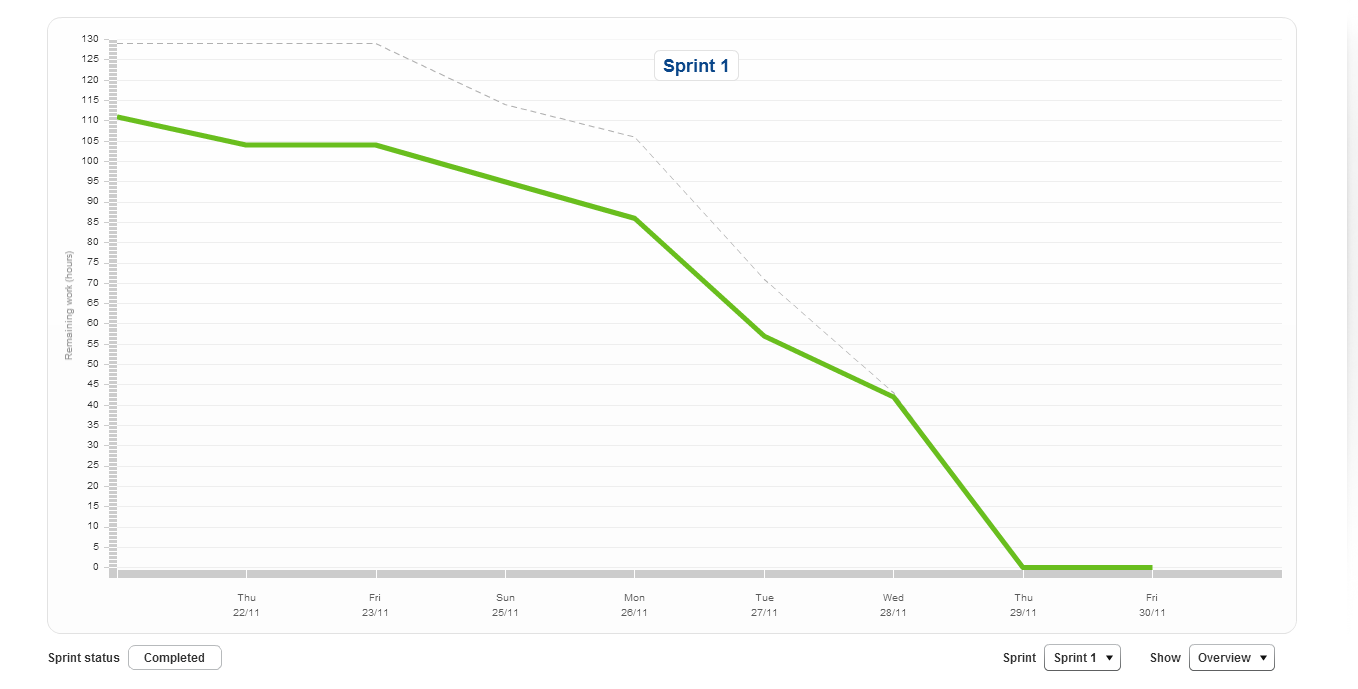
\includegraphics[width=\textwidth,natwidth=1253,natheight=673]{illustrations/burndown.png}
  \caption{Sprint 1 Burndown Chart}
  \label{sprint1burnchart}
\end{figure}
The final scrum activities we’ll discuss is the inspect and adapt related meetings at the end of a sprint. However, in order to maintain our chronological order of the report, we’ll defer the discussion of additional scrum-related activities such as: Scrum Retrospective and Scrum Review to the end of this sprint documentation.\\
\newpage